\appendix
\chapter{Requirements}
\vspace{-1cm}
\epigraph{\textbf{Author: } Markus Just, Wojciech Lesnianski}
 
\vspace{-1cm}
\section{Top-Level-Requirement}
The application should bring out a car from different parking positions
automatically.

\section{Functional Requirements}

\textbf{Required}

\begin{longtable}[l]{p{0.1\textwidth}p{0.8\textwidth}}
\textbf{A.2.1} & The application should be able to bring out the car from a parallel parking position\\
\textbf{A.2.2} & The application should be able to bring out the car from a perpendicular parking position\\
\textbf{A.2.3} & The application should be able to bring out the car from an angled parking position\\
\textbf{A.2.4} & The application should be able to work on the road side\\
\textbf{A.2.5} & The application should be able to work in a parking facility\\
\textbf{A.2.6} & The application should provide relevant sensor information to the driver in an graphical overview\\
\textbf{A.2.7} & The application should provide information about the current action to the driver in an aerial car view\\
\textbf{A.2.8} & It should always be possible for the driver to intervene the current process\\
\textbf{A.2.9} & The application should be able to work with right-hand traffic\\
\textbf{A.2.10} & The application should be able to work with left-hand traffic\\
\textbf{A.2.11} & The application should consider the traffic rules and should act properly\\
\textbf{A.2.12} & The application should bring the car out of the parking system in a way that after that process it is possible to enter it from all sides\\
\end{longtable}

\begin{raggedleft}
\textbf{Nice-to-have}
\end{raggedleft}

\begin{longtable}[l]{p{0.1\textwidth}p{0.8\textwidth}}
\textbf{A.2.13} & The application should work independent of the current weather conditions\\
\textbf{A.2.14} & The cars should have customizable skins, selectable by the user\\
\textbf{A.2.15} & The application should be remote-controllable by a mobile application if the user is within a defined range to the vehicle\\
\end{longtable}

\section{Non-functional Requirements}

\begin{longtable}[l]{p{0.1\textwidth}p{0.8\textwidth}}
\textbf{A.3.1} & The application must comply national safety regulations\\
\textbf{A.3.2} & The application should have a suitable design\\
\textbf{A.3.3} & The application should be integrated in the given car's entertainment system\\
\textbf{A.3.4} & The application's GUI should be easy to grasp for the user\\
\textbf{A.3.5} & The application should be easy to extend\\
\textbf{A.3.6} & The application should be secured against any kind of attack\\
\textbf{A.3.7} & The application should be integrateable in different sorts of vehicles\\
\textbf{A.3.8} & The application should be developed with C\#/.NET\\
\textbf{A.3.9} & The application�s GUI should be developed with WPF.\\
\end{longtable}


\chapter{PERT-Diagram}
\label{sec:pert}
\vspace{-1cm}
\epigraph{\textbf{Author: } Markus Just}
 
\vspace{-1cm}

\begin{figure}[h!]
  \centering
     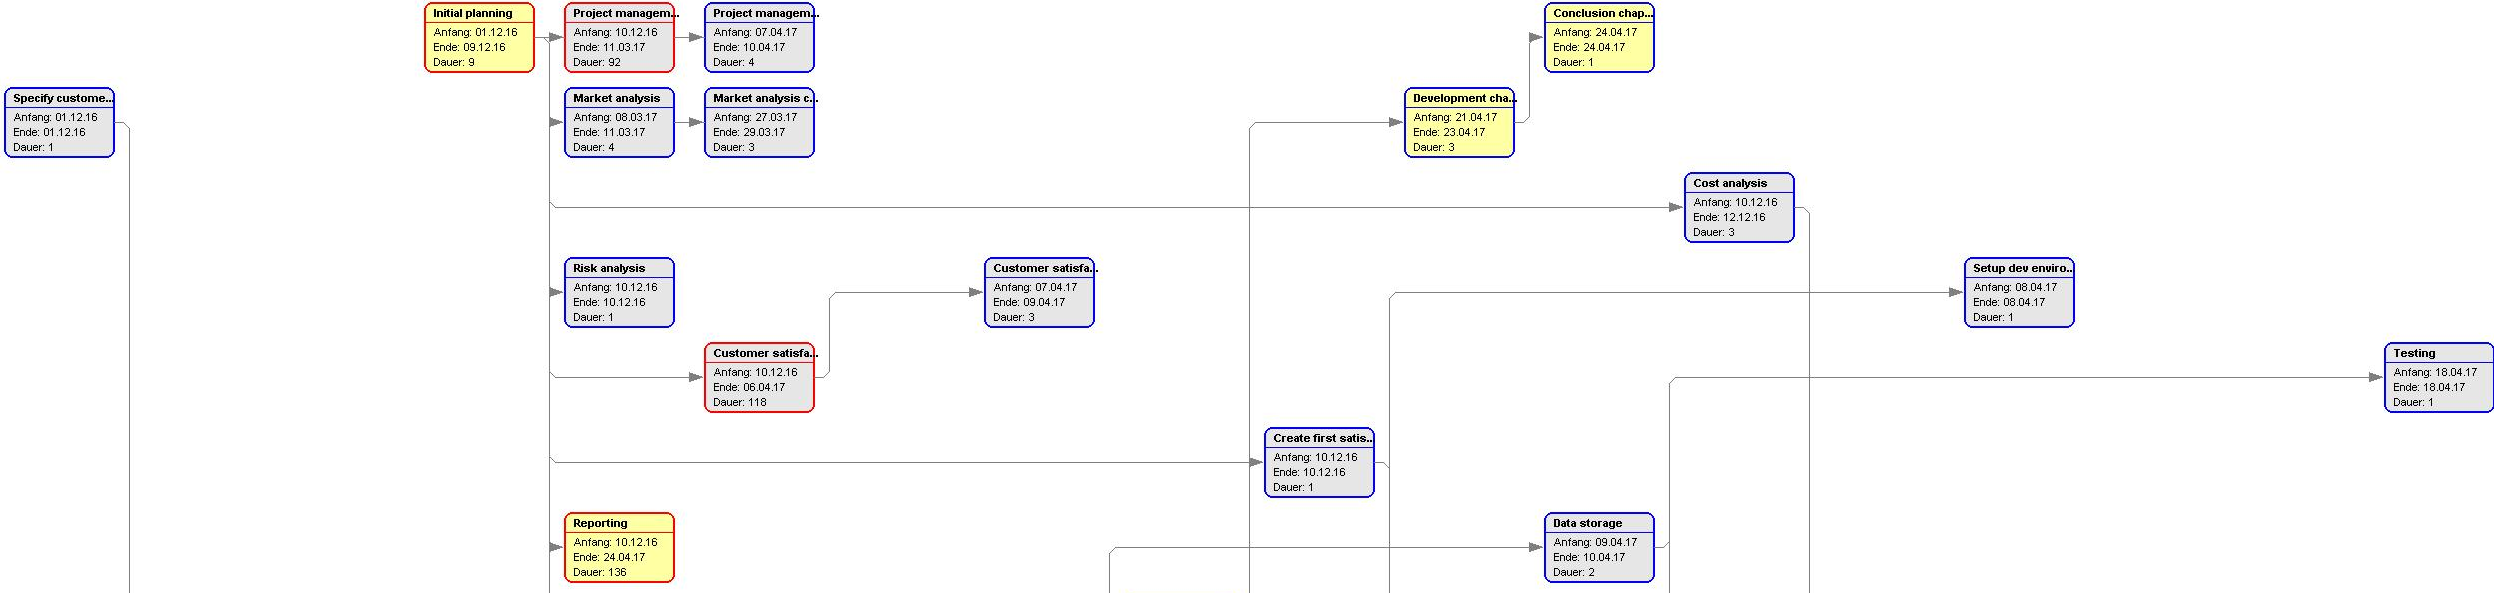
\includegraphics[width=0.95\textheight, height= 0.3\textwidth,angle=90]
     {res/projectPlan/pert1.png}
     \captionsetup{justification=centering}
  \caption{PERT-Diagram Full (1/3)}
  \label{fig:full pert}
\end{figure}

\begin{figure}[h!]
  \centering
     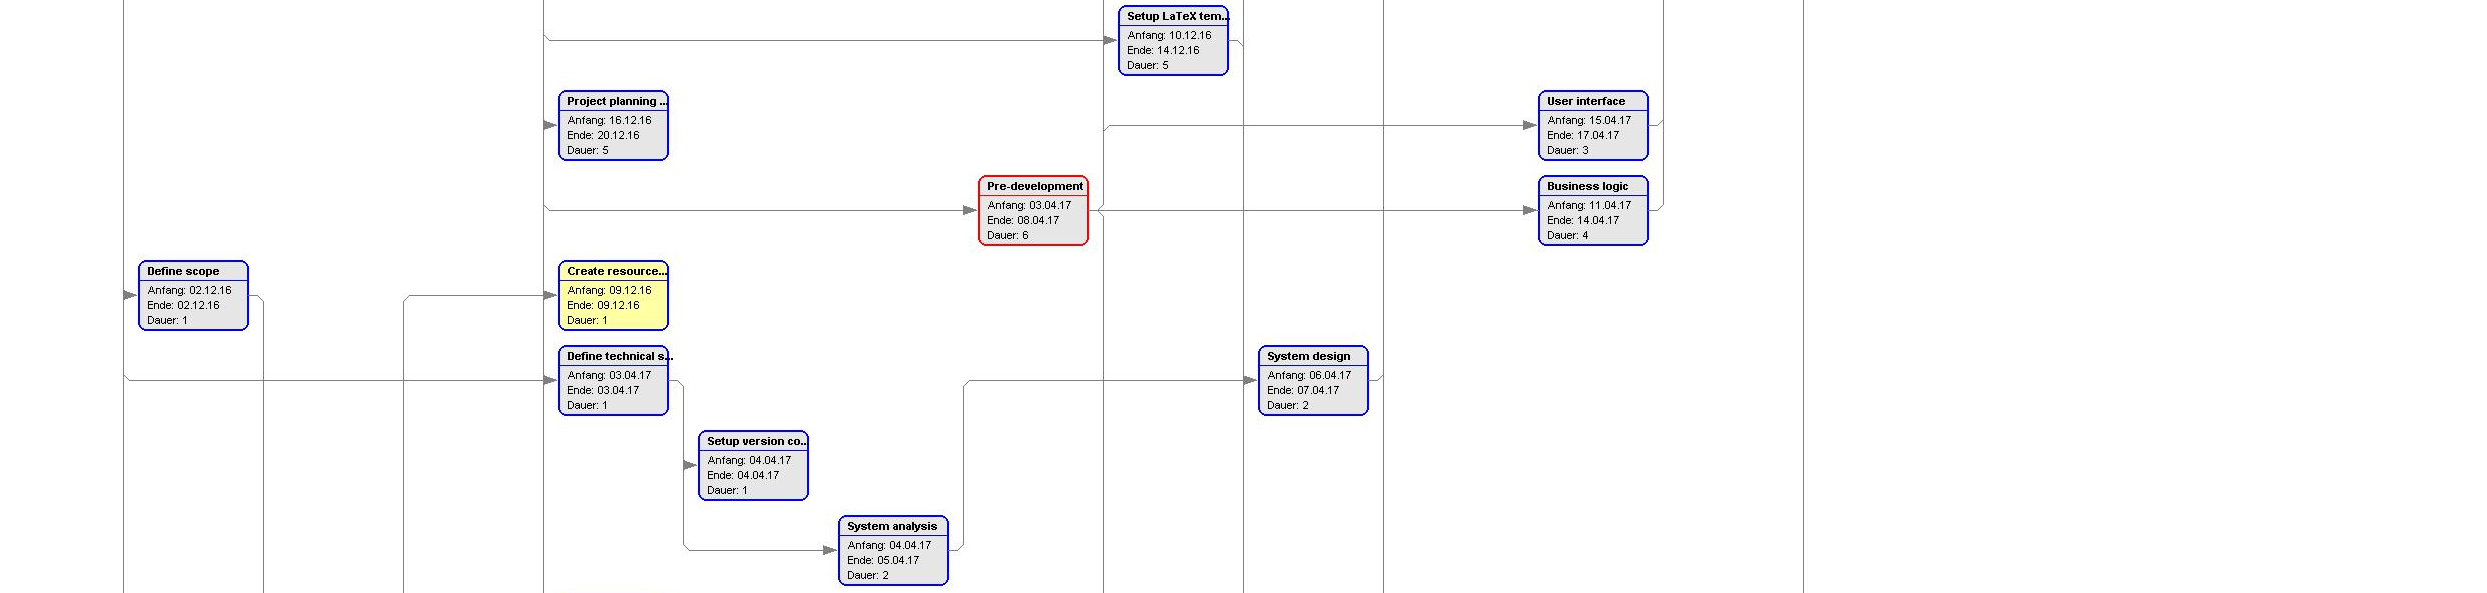
\includegraphics[width=0.95\textheight, height= 0.3\textwidth,angle=90]
     {res/projectPlan/pert2.png}
     \captionsetup{justification=centering}
  \caption{PERT-Diagram Full (1/3)}
  \label{fig:full pert}
\end{figure}

\begin{figure}[h!]
  \centering
     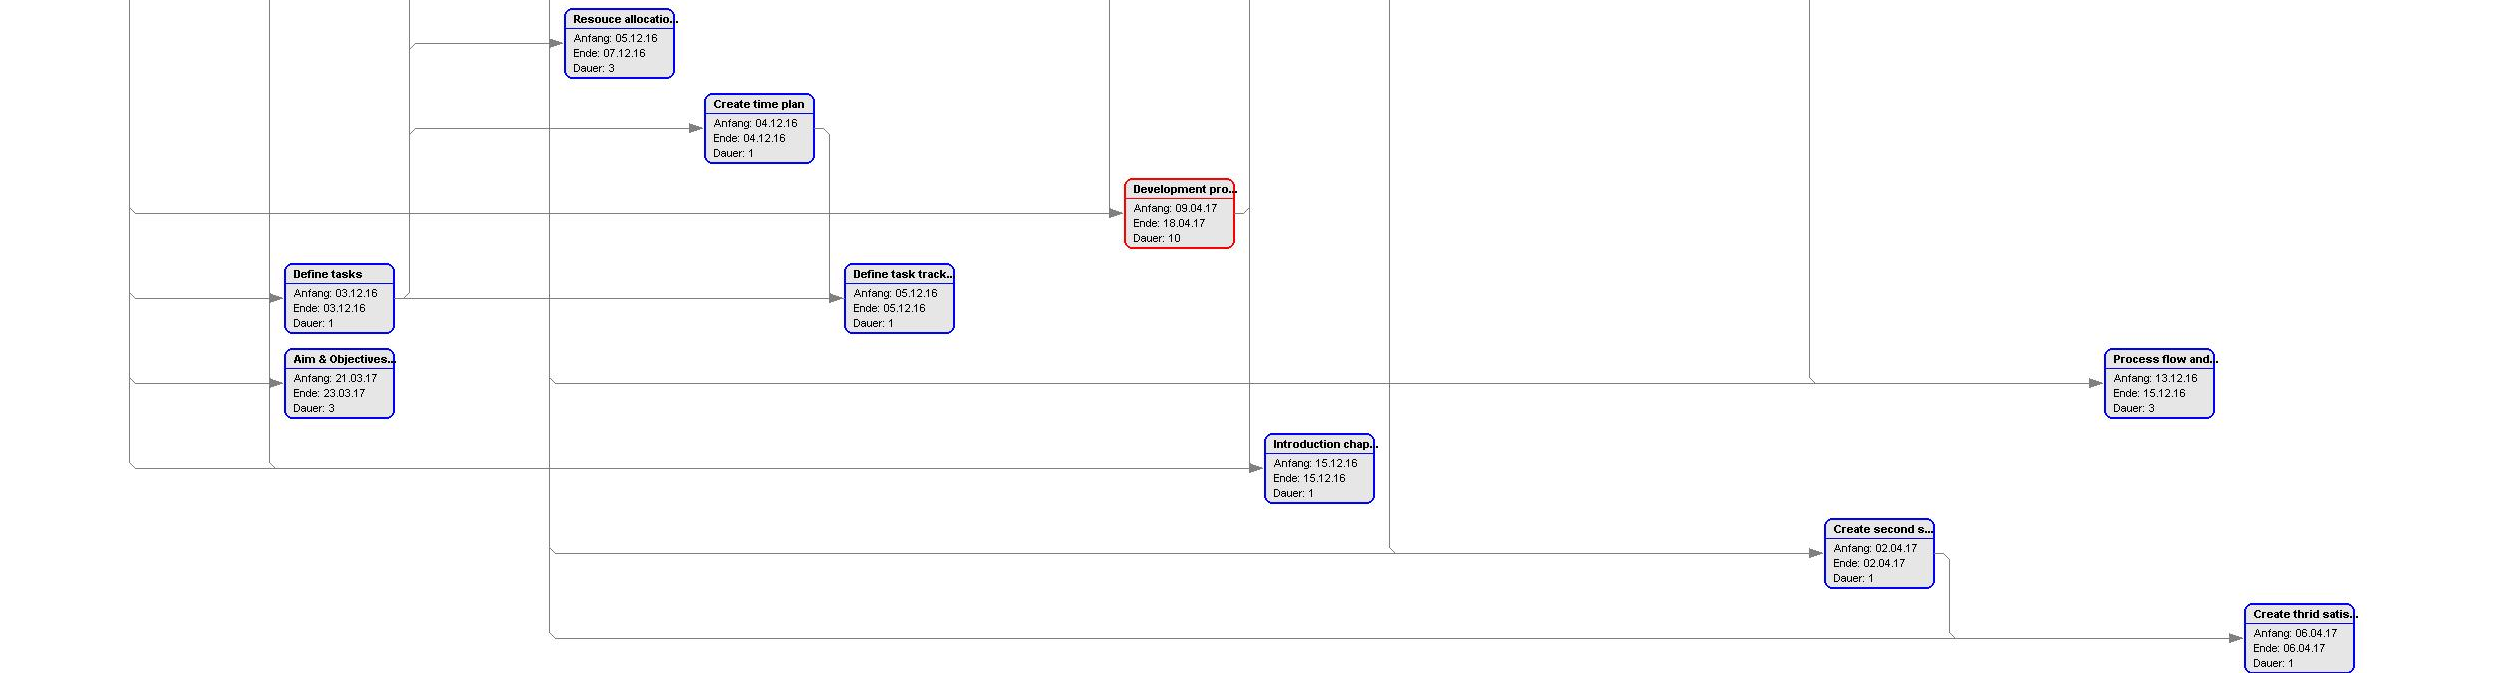
\includegraphics[width=0.95\textheight, height= 0.3\textwidth,angle=90]
     {res/projectPlan/pert3.png}
     \captionsetup{justification=centering}
  \caption{PERT-Diagram Full (1/3)}
  \label{fig:full pert}
\end{figure}

